In this section, we briefly introduce the concepts of key exchange, Federated Learning, multi-party computation and Consensus Algorithms, which are used in our proposed framework.

\subsection{Key Exchange}
Key exchange protocols allow several parties to share secret keys under unsafe conditions. Diffie-Hellman~\cite{DH} (DH) is a prestigious key exchange protocol. We introduce how DH protocol helps two parties to achieve agreement: suppose $a$ and $b$ want to obtain a secret key by means of DH. First they select a group $G$ of order q, and randomly choose a number $x_a$ and $x_b$ respectively. Then $a$ calculates $g_a = g^{x_a}$, where $g$ is a generator of $G$, and $b$ calculates $g_b = g^{x_b}$. $a$ sends $g_a$ to $b$, and $b$ sends $g_b$ to $a$. Finally they can calculate the shared secret $s_{ab}$ respectively:
$$ s_{ab} = g_b^{x_a}  = g_a^{x_b} = g^{x_ax_b}$$

In this scheme, only $g_a$ and $g_b$ are sent under an unsafe condition. Attackers cannot infer $s_{ab}$ from $g_a$ and $g_b$, therefore $a$ and $b$ can communicate privately by means of $s_{ab}$. DH is lightweight and efficient, and it can be expanded to multi-party versions easily in order to enable more parties to share pairwise keys.


\subsection{Federated Learning}
Federated Learning was first proposed by McMahan and the algorithm was named FedAvg~\cite{mcmahan2016communicationefficient}. FL requires a number of users to jointly train a model. It usually runs for rounds. In each round, each user will train the model based on its data and get the model's parameter. Mark $W_i^t$ as the $i^{th}$ user's parameter in the $t^{th}$ round. When all users have trained their model in round $t$, an aggregation algorithm $Agg$ will be called to compute the global model's parameter $Agg(W_1^t, W_2^t, ..., W_n^t)$, where $n$ is the total number of users. $Agg$ is weighted average in FedAvg. FL not only helps to protect users' privacy but also deals with the ``data in form of isolated islands'' problem for companies or institutions. Yang et al. also categorized FL into horizontal, vertical and hybrid styles based on the fact that whether the data shares the same feature space or entities~\cite{yang2019federated}. 

Federated Learning can be generalized to two work environments:

\begin{enumerate}

    \item \textbf{Among-institutions:} In this situation FL is usually used to help companies or other institutions solving the ``data in form of isolated islands'' problem. Generally, companies and institutions are in equal status in an FL framework. Therefore, we can suppose one party can communicate with any other one privately. I.e., P2P is already enabled in this environment.

    \item \textbf{Server based:} In this case a company or institution adopts FL to train a model based on their users' data while protecting their privacy. An FL party is a common user, which means users' communication usually needs to go through the server. With an honest-but-curious server, all information will be eavesdropped by it. Therefore, the problem with confidence is severe in such environments.

\end{enumerate}

Figure~\ref{fl_model} illustrates the structures of two environments. Executing MPC protocols and consensus algorithms are at a low price in the first environment. In the second environment, if local parameters need to be protected, we need to run some key-exchange protocols first to construct secure channels among users. Google's keyboard query suggestions~\cite{yang2018applied} project was an effective application of server-based federated learning. One of our contribution is that we solved the problem in the second environment by building connections selectively and efficiently.


\begin{figure}[!ht]
    \centering
    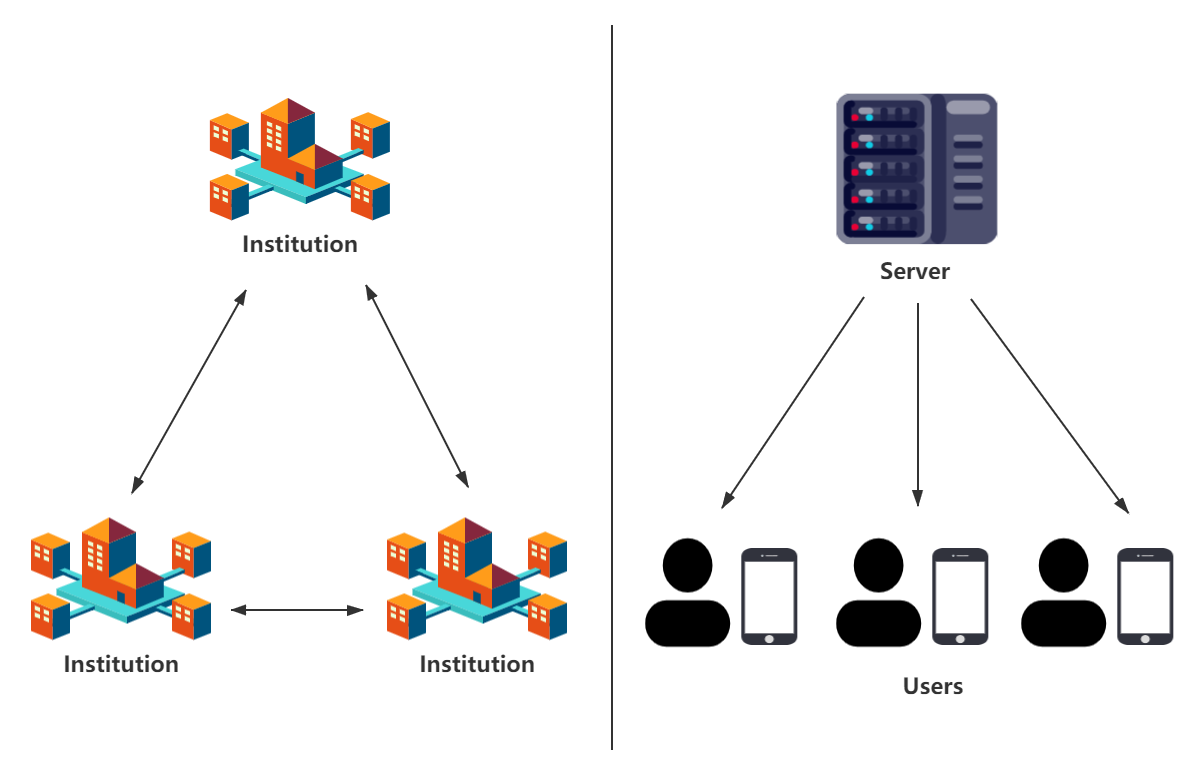
\includegraphics[width=\columnwidth]{img/fl_model.png}
    \caption{The structures of 2 work environments in Federated Learning. The left is the ``Among-institutions'' model where institutions can communicate with others directly, and the right is ``Server based'' model where parties exchange information in virtue of the server.}
    \label{fl_model}
\end{figure}


\subsection{Multi-party Computation}
Secure MPC is a branch of cryptography which enables several parties to compute a particular function without leaking their own data (inputs). Suppose there are $n$ parties employing MPC to compute a function $F$, and the $i^{th}$ party has its parameter $A_i$. Their goal is to compute $R = F(A_1, A_2, ..., A_n)$. MPC has the feature that participants can only obtain $R$ from the process and the party $P_i$ has no idea about parameter $A_j (j \ne i)$. This feature fits the aggregation algorithm in FL greatly.

It was first proposed by Yao to solve the millionaire problem~\cite{Yao}. Most MPC protocols depend on two cryptography technologies: secret sharing~\cite{Shamir} and oblivious transfer~\cite{OT}. MPC can be implemented with garbled circuits, multi-party circuit-based protocols or hybrid methods~\cite{mpc-sok}. It also benefits from fully homomorphic encryption (FHE) algorithms. Garbled circuits and FHE suffer from complicated design and poor efficiency. Therefore, secret sharing methods are more favored to solve the privacy-preserving problem in FL. SPDZ~\cite{SPDZ} (speedz) is a practical and secure MPC protocol introduced by Damgard et al. It supports addition and multiplication by means of the triples~\cite{Triple}, which are generated by somewhat homomorphic encryption (SHE). Our method does not require multiplication and hence we do not need to generate the triples choose to use simple additive MPC.

A secret sharing scheme involves a secret $s$, a set of $n$ parties, and a collection $A$ of subsets of parties. Each party has its share of $s$. The secret sharing scheme ensures any subset in $A$ can reconstruct $s$~\cite{Secret-Sharing-survey}. By means of secret sharing, we can implement secure addition among parties, which is essential in our framework.


\subsection{Consensus Algorithms}
In a distributed or multi-party system, there is always a problem with consensus. I.e., in such systems parties always need to achieve agreement on a certain value. This could be difficult without any strategy because different parties may be in different statuses and have multifarious matters. Consensus algorithms are adopted to address such problems. It is widely used in blockchain and various famous areas.

Paxos was the first consensus algorithm introduced by Lamport~\cite{Paxos}. It is used in a lot of famous projects such as Ceph~\cite{Ceph}. Raft is a modification of Paxos which is more industrial-friendly~\cite{Raft}. It contains two phases: leader election and log replication. Parties can achieve agreements based on leaders. Considering that FL model is a semi-decentralized system, our framework can utilize Raft algorithm to keep several leaders, based on which MPC protocols can be executed efficiently and robustly.
